\chapter{\label{chapter:background}Background in Embedded Systems and Virtualization}


This chapter explains basic concepts to better understand the remainder of the text. Virtualization is a complex subject that involves several different topics and a wide range of solutions. This dissertation focuses on virtualization for the embedded systems. Thus, Section \ref{section:es} starts by explaining the concept of embedded systems. If the reader is familiar with the definition of embedded systems, it is suggested that you read this chapter from Section \ref{section:envirt}. Section \ref{section:virtualization} introduces virtualization and its taxonomy, the different types of hypervisors and the requirements for virtualization. Section \ref{section:envirt} explains different technologies that make virtualization possible. Section \ref{section:virt_challenges} describes two different problems caused by the use of virtualization. Section \ref{section:ev} shows the advantages of virtualization for embedded systems. Finally, Section \ref{section2:future} discusses the past, present and future of virtualization for embedded systems. If you are familiar with virtualization and embedded virtualization concepts, it is suggested to read this work from Chapter \ref{chapter:stateofart}.

\section{Embedded Systems}
\label{section:es}

The use of microprocessors in equipment and consumer applications rather than laptop or personal computers (PCs) is wide spread. Actually, PCs are only one application of microprocessors. Embedded microprocessors are deeply integrated into everyday life, i.e., cars, microwaves oven, TVs, cell phones, and many other electronics are powered by microprocessors. Additionally, the increasing adoption of Internet of Things (IoT) \cite{gubbi2013} is accelerating the use of embedded applications. It is expected that there will be 24 billion interconnected devices by the year 2020 \cite{gubbi2013}. 

An embedded system (ES) is a computer system designed for a specific purpose, which  distinguishes it from PCs or supercomputers. However, it is difficult to find a unique definition for ESs as they constantly evolve with advances in technology and as costs decrease. The following definition from \cite{heath2003} says: \textit{An embedded system is a microprocessor-based system that is built to control a function or range of functions and is not designed to be programmed by the end user in the same way that a PC is}. Most embedded devices are designed for a specific function. However, this definition sounds outdated as modern ESs may allow the final user to develop and download new applications, e.g., smartphones and smartTVs. Additionally, another definition highlights  their  reliability \cite{Noergaard2005}: \textit{An ES is a computer system with higher quality and reliability requirements than other types of computer systems.} This definition covers systems such as avionics or medical equipment where a malfunction is  life-threatening. Due to the wide range of ES purposes, there is not a single definition. Table \ref{table:esMarket} shows examples of the embedded system markets and devices.  

\begin{table}[!hbtp]
\centering
\caption{Example of embedded systems market and devices. Adapted from \cite{Noergaard2005}.}
\label{table:esMarket}
\begin{tabular}{|p{6cm}|p{5cm}|}
\hline
\textbf{Market}               & \textbf{Embedded Device}                                                                            \\ \hline
Automotive           & \begin{tabular}[c]{@{}l@{}}Ignition system\\ Air bag sensors\\ Engine control\end{tabular} \\ \hline
Consumer electronics & \begin{tabular}[c]{@{}l@{}}Smart phones\\ Smart TVs\\ Games\\ Toys\\ Laptops\end{tabular}   \\ \hline
Industrial control   & Robotics                                                                                   \\ \hline
Medical              & \begin{tabular}[c]{@{}l@{}}Cardiac monitors\\ Dialysis machines\end{tabular}               \\ \hline
Networking           & \begin{tabular}[c]{@{}l@{}}Routers\\ Switches\end{tabular}                                 \\ \hline
Office automation    & \begin{tabular}[c]{@{}l@{}}Printers\\ Scanners\end{tabular}                                \\ \hline
\end{tabular}
\end{table}


A recent trend in ESs is about  their software complexity. Noergaard \cite{Noergaard2005} defined ES software and application layers as optional. Thus, an ES could be composed of only a hardware layer. However, the performance improvement in functionalities, processing power and storage capacity over the last years has enabled a wide range of new complex applications and functionalities for ESs. Thus, the designers tend to adopt complex software layers to accomplish their goals. As mentioned  early in this section, the possibility for the final user to develop and download new applications, before exclusively found in general-purpose systems, can now be found in many embedded devices. This has  forced designers and companies to adopt new strategies, resulting in the increased use of software layers.

Although ESs are incorporating general-purpose features, many constraints remain. Because they are designed for specific functions, engineers can reduce the size and cost of the final product resulting in relatively simple and cheap devices. Thus, ES may suffer from hardware constraints, like reduced processing power, memory, weight and battery life. This added to the increasing complexity of embedded software is a challenge for designers that still need to meet timing, energy consumption, and time-to-market constraints for their products. In this scenario, virtualization can be a useful tool to deal with software complexity while increasing reuse, security and software quality. 


\section{What Means Virtualization?}
\label{section:virtualization}

Virtualization means the creation of an environment or, the creation of a virtual machine (VM), that acts like the real target hardware from the software or user point of view. The VM is implemented as a combination of real hardware and software aiming to execute applications \cite{Smith2005}. Figure \ref{fig:taxonomy} depicts the taxonomy of VMs suggested by \cite{Smith2005}. There are two kinds of VMs: process VMs and system VMs. Typically, a process VM is implemented on top of the operating system's (OS) application binary interface (ABI) and is able to emulate both user-level instructions and OS system calls for an individual process. A system VM provides a complete system environment capable of  supporting an entire OS. Thus, a single computer can support multiple \textit{guest OSs} environments simultaneously. A guest OS is an OS executing inside of a VM, i.e., a virtualized OS. In this dissertation, the term guest OS will be used to distinguish between virtualized and non-virtualized OSs. The second taxonomy level is based on whether the guest and host execute the same instruction set architecture (ISA). Multiprogrammed OSs are a typical example of process VMs that execute the same ISA. Process VMs for different ISA needs to emulate program binaries compiled to a different ISA. Two techniques can be applied to perform emulation: 

\begin{itemize}
  \item Interpretation: Fetches, decodes and emulates the execution of individual source instructions. This technique results in a huge performance impact because each instruction requires many native instructions to be emulated.
  \item Dynamic Binary Translation: Blocks of source instructions are translated into native instructions. This technique increases the performance because the translated blocks can be cached and repeatedly executed without requiring new translation. 
\end{itemize}


\begin{figure}[!hbtp]
	\centering
	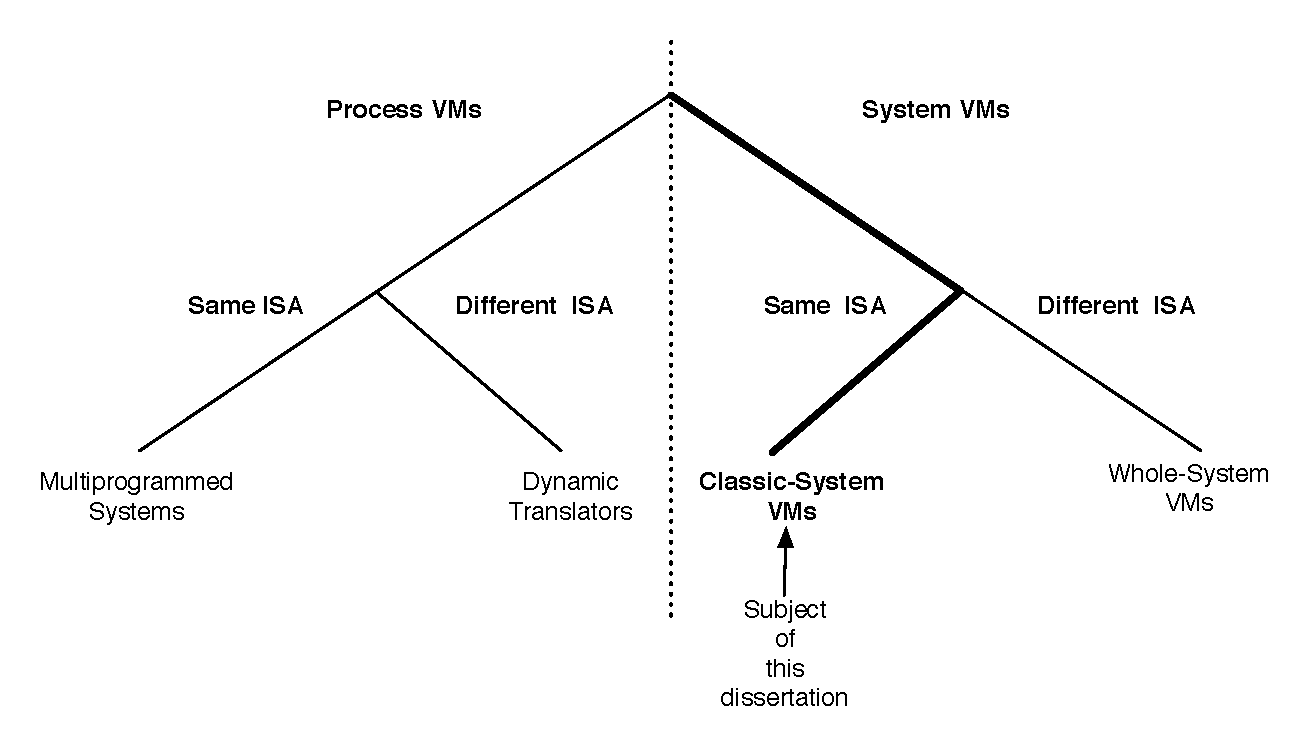
\includegraphics[width=0.7\textwidth]{chapter2/figures/taxonomy}
	\caption{A taxonomy of Virtual Machines. Classic-system VMs are the subject of study of this dissertation. Adapted from \cite{Smith2005}.}
	\label{fig:taxonomy}
\end{figure}


Interpretation and binary translation have different performance profiles \cite{Smith2005}. Interpretation has lower startup overhead but greater overhead for overall execution. On the other hand, binary translation has high initial overhead in order to translate the instructions for the first time. Thus, some VMs use both techniques combined with a heuristic to determine which source instruction blocks will be interpreted or translated. The best example of a process virtual machine is the Java Virtual Machine \cite{Lindholm1999}. Java is a high-level language (HLL) designed for portability. The Java compiler generates a portable intermediate ISA that can be emulated by the Java Virtual Machine (JVM) for different host ISAs. 

In system VMs, the virtualization software is often called a \emph{virtual machine monitor} (VMM) or simply \emph{hypervisor}. System VMs designed to support different ISAs need to emulate all software (OSs and applications). Thus, they are also called whole-system VMs. There are important applications for this kind of VM. For example, an ARM platform including the processor, memory and peripherals can be fully emulated on an Intel IA-32 processor. Thus, the designers can test their software without the target hardware. Additionally, a legacy software can be supported by newer platforms without requiring engineering work to port. An example of a system VM for different ISAs is the QEMU \cite{qemu}. QEMU is an open source application that can be used either as an emulator or virtualizer. As an emulator, it can run OSs and programs compiled for different ISAs. When used as a virtualizer, it can execute the guest OS code directly on the host CPU. Another example is Open Virtual Platforms (OVP)\footnote{http://www.ovpworld.org/} designed to accelerate embedded software development allowing hardware platforms to be described in C language. Thus, the designers can describe their custom platform, testing and debug their software without the real target. 

System VMs to the same ISA, also called classic-system VMs, were developed during the 1960s and they were the first application of virtual machines. At that time, mainframe computer systems were large and expensive. Thus, computers needed to be shared among users. Different users sometimes required different OSs creating the first practical application for virtualization. With the popularization of PCs, interest in classic-system VMs was lost. However, during the 1990s with the appearance of server farms, the classic-system virtualization became popular once again. In this case servers are shared among several users and VMs are a secure way of partitioning the user's software. Classic-system VMs have a lower performance impact when compared to whole-system VMs because the hardware directly executes the VM's instructions.

Recently, the interest in classic-system VMs for embedded systems has increased. However, classic-system VM as applied to server virtualization does not fit directly with ESs. Their intrinsic characteristics as discussed in Section \ref{section:es} motivated the study of new approaches for virtualization on ESs. Thus, the subject of this dissertation is classic-system VMs for embedded systems. Hereafter, the term virtual machine refers to classic-system VMs, unless otherwise noted. 


\subsection{Types of Hypervisors}
\label{subsection:hypertypes}
%procurar referencia para os termos type 1 e type 2.

Virtualizing software (VMM or hypervisor) can be divided into two different kinds called \emph{type 1} and \emph{type 2}. Figure \ref{fig:hyper_types} depicts both. Type 1 hypervisors are also called \emph{native} or \emph{bare-metal} hypervisors. The virtualization layer is implemented between the hardware and the guest OSs, i.e., there is no native OS executing in a system that adopts type 1 virtualization as shown in Figure \ref{fig:hyper_type1}. A representative type 1 hypervisor is Xen (see Section \ref{section:xen}). A type 2 hypervisor is implemented as a distinct software layer on top of an existing OS  (see Figure \ref{fig:hyper_type2}). From the point of view of the underlying OS, it is treated as a normal process and is subject to the same scheduler policies as other user and system processes. In this kind of virtualization, a guest OS can coexist along with the non-virtualized user processes. A representative type 2 hypervisor is KVM (see Section \ref{section:kvm}).

When a home/office user desires to utilize virtualization for some purpose, type 2 hypervisors are most popular. The type 2 hypervisor is installed as a user's application on the existing OS. This technique allows the user to execute a guest OS along with other user applications. Thus, the guest OS is competing with user applications for system resources, and it is submitted to the same host OS policies as any other process. In terms of memory requirements, type 1 hypervisors are more efficient than type 2 since there is not the overhead of the host OS. Additionally, the hypervisor has the freedom to control all system resources. The main application for type 1 hypervisors is to execute multiple OSs on the same computer, which makes it the perfect choice for server consolidation. 

\begin{figure}[!hbtp]
\centering
\subfigure[Type 1 hypervisor.]{
	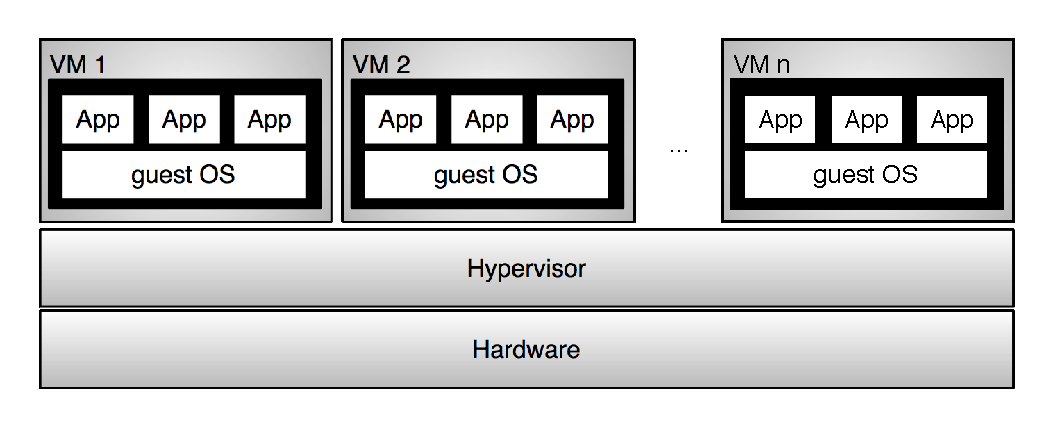
\includegraphics[width=.70\textwidth]{./chapter2/figures/hyper_type1}
	\label{fig:hyper_type1}}
\quad

\subfigure[Type 2 hypervisor.]{
	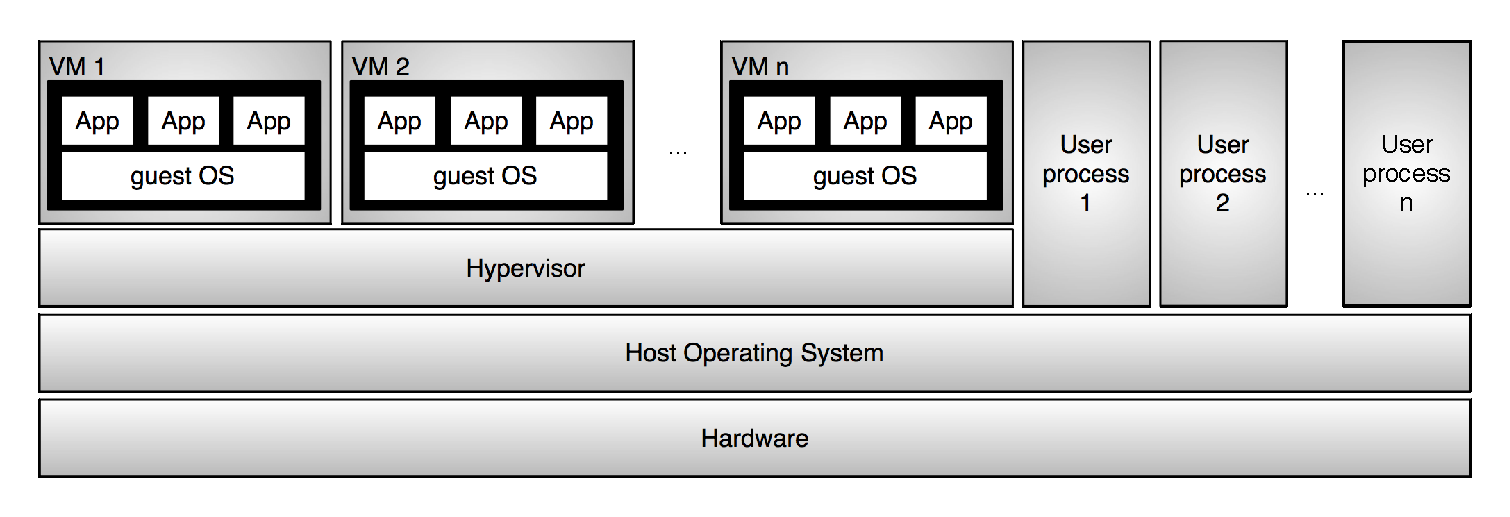
\includegraphics[width=.70\textwidth]{./chapter2/figures/hyper_type2}
	\label{fig:hyper_type2}}
\caption{Types of hypervisors.}
\label{fig:hyper_types}
\end{figure}

Type 1 and type 2 hypervisors are available for embedded virtualization. However, most type 2 hypervisors used in embedded virtualization were designed for desktop virtualization and adapted for embedded systems. As presented in the Chapter \ref{chapter:stateofart}, hypervisors designed specifically for embedded systems tend to implement the type 1 approach. Due to restrictions such as memory footprint and real-time constraints, the type 1 model fits embedded systems better. The virtualization model for ESs proposed in this dissertation depicts a type 1 hypervisor. 


\subsection{Requirements for Processor's Virtualization}
\label{subsection:vz-requirements}

The classic paper written by Popek and Goldberg \cite{Popek1974} formalizes the conditions for a processor architecture to be efficiently virtualized. Efficient  virtualization means  that a VM can be constructed over the processor's architecture without the necessity of modifying the guest OS. In order to understand their theorem, it is necessary to define the difference between control-sensitive, behavior-sensitive and privileged instructions. Control-sensitive instructions can change the configuration of the system's resources, while, behavior-sensitive instructions depend on the configuration of the resources. Instructions that are neither control-sensitive nor behavior-sensitive are termed innocuous \cite{Smith2005}. Moreover, instructions that trap the OS when executed in user mode are called privileged instructions. In a hypervisor, any instruction that attempts to change the configuration of the system's resources must be intercepted and emulated accordingly. This is possible when two requirements are accomplished: 

\begin{itemize}
  \item The instruction was executed in user-mode and;
  \item The control-sensitive and behavior-sensitive instructions are privileged instructions too. 
\end{itemize}  

The first requirement is easily accomplished executing the hypervisor in kernel-mode and the guest OS in user-mode. However, the second requirement relies on the processor's architecture. Thus, Popek and Goldberg stated their theorem:

\begin{thm}
"For any conventional processor a virtual hypervisor may be constructed if the set of sensitive instructions for that computer is a subset of the set of privileged instructions.
\end{thm}

Figure \ref{fig:sensitive_instr} depicts the theorem. In  Figure \ref{fig:sensitive_instr1} the control-sensitive instructions are not a subset of the privileged instructions, i.e., some of them can be executed in user-mode without trapping the hypervisor. This case violates Popek-Goldberg's theorem and cannot be efficiently virtualized.  On the other hand, Figure \ref{fig:sensitive_instr2} shows the control-sensitive instructions as a subset of the privileged instructions resulting in a processor that can be efficiently virtualized.

\begin{figure}[!hbtp]
\centering
\subfigure[Not efficiently virtualizable.]{
	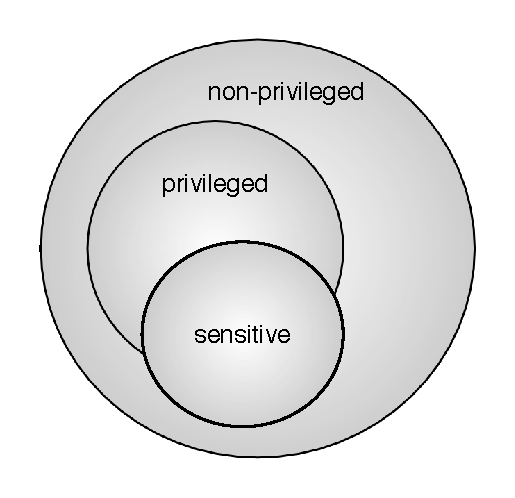
\includegraphics[width=.4\textwidth]{./chapter2/figures/sensitive_instr1}
	\label{fig:sensitive_instr1}}
\quad
\subfigure[Efficiently virtualizable.]{
	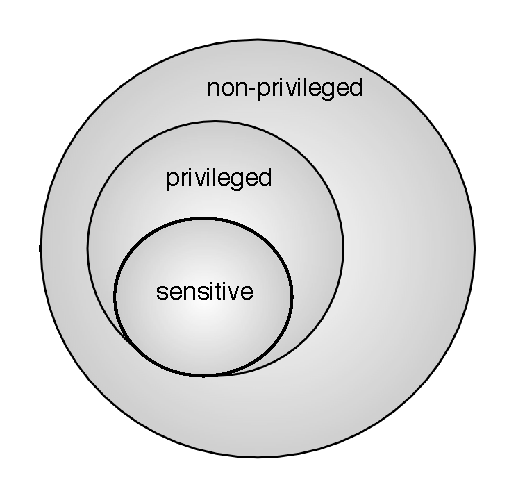
\includegraphics[width=.4\textwidth]{./chapter2/figures/sensitive_instr2}
	\label{fig:sensitive_instr2}}
\caption{Illustrating Popek and Goldbergs's Theorem. Adapted from \cite{Smith2005}.}
\label{fig:sensitive_instr}
\end{figure}

Para-virtualization (see Subsection \ref{subsection:paravirt}) can be applied when the processor's architecture is not compatible with the Popek-Goldberg theorem. Thus, allowing a hypervisor  implementation for that architecture. Alternatively, processors that support Popek-Goldberg’s theorem can be fully-virtualized (see Subsection \ref{subsection:fullvirt}). Section \ref{section:envirt} explains the difference between para-virtualization, full-virtualization and hardware-assisted virtualization. 


\section{Enabling Techniques and Technologies for Virtualization}
\label{section:envirt}

The evolution of virtualization technology has resulted in several different ap\-proach\-es. The variety of processor architectures and the appearance of new applications with different needs, has driven  techniques that can deliver virtualization on almost all devices. This section describes the three main techniques adopted for hypervisor implementation: para-virtualization (Subsection: \ref{subsection:paravirt}), full-virtualization (Subsection \ref{subsection:fullvirt}) and hardware-assisted virtualization (Subsection \ref{subsection:hardware-assisted}).  These techniques can be adopted separately or  through a hybrid approach, combining two or more of them. The virtualization model and the resulting hypervisor implementation, which is the subject of this work, are a combination of these three techniques.

\subsection{Para-virtualization}
\label{subsection:paravirt}

Hypervisors for processor architectures that do not fit Popek and Goldberg’s theorem, as explained in Subsection \ref{subsection:vz-requirements}, require different approaches. These architectures have control-sensitive instructions that do not trap the hypervisor. Therefore,  the hypervisor cannot avoid an application changing the processor's behavior. There are two ways to avoid this problem: dynamic binary translation or para-virtualization (PV). Hypervisors that perform dynamic binary translation need to read the VM's instruction prior to their execution in order to emulate the control-sensitive instructions that do not trap the hypervisor. Thus, causing a significant performance penalty when compared to PV. Para-virtualization is a technique that requires modifying and recompiling the guest OS prior to its installation in a VM. These modifications consist of substituting control-sensitive instructions or other OS parts, like the I/O subsystem, by hypercalls. However, for proprietary software or other situations where the source code is not available, the only alternative is dynamic binary translation.  

Hypercalls are services provided by the hypervisor and invoked from the guest OS. They are equivalent to system calls (syscalls) in an OS and Figure \ref{fig:syscall} describes their relationship. In operating systems, functions that can only be performed by the OS, like memory allocation or access to the file-system, result in calls to the OS. Similarly, functions that can only be performed by the hypervisor, such as the execution of control-sensitive instructions, can be converted to hypercalls. 

\begin{figure}[!hbtp]
	\centering
	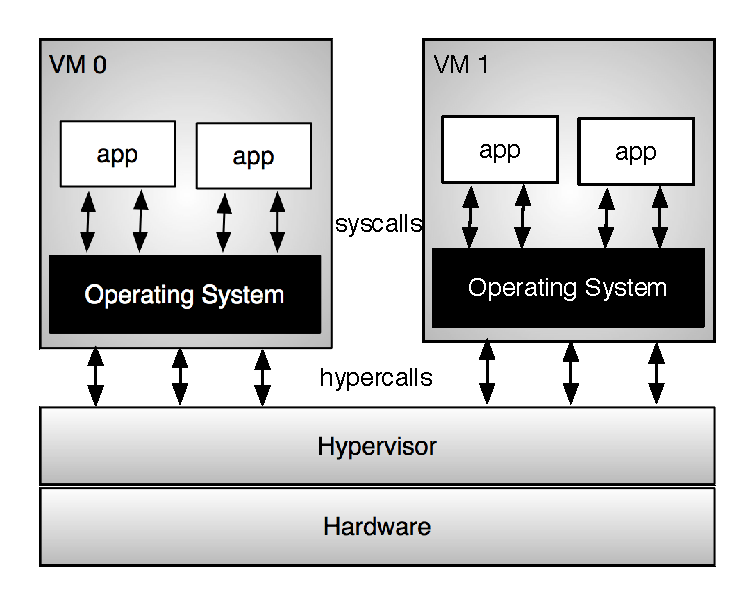
\includegraphics[width=.45\textwidth]{chapter2/figures/syscall}
	\caption{Relation between hypercalls on a virtualized system and syscalls on a typical operating system.}
	\label{fig:syscall}
\end{figure}

PV is not limited to processor architectures that cannot support Popek and Goldberg’s theorem. In fact, it can extend hypervisor capabilities. For example, PV can be used to implement communication between the VM and the hypervisor or inter-VM communication. Another application for PV is to improve performance, since fully-virtualized hypervisors have a performance issue. If the VM executes control-sensitive instructions constantly, it will result in an excessive number of traps to the hypervisor, impacting performance. Thus, the OS can be modified to substitute these instructions with hypercalls.  

The main limitation of para-virtualization is the engineering work needed to modify the OS to execute in a specific hypervisor. When utilized as a method to extend the capabilities of a virtualized platform, e.g., to support inter-VM communication, PV can be applied as a loadable module. Usually modern operating systems support kernel modules \cite{rubini2005}, i.e., executable code that can be dynamically loaded into an OS's kernel to add new functionalities. For example, an inter-VM communication module can be added without modifying the OS's source code. VirtIO \cite{Russell2008} is a effort to standardize the I/O interfaces for Linux hypervisors consisting of a set of Linux modules. However, para-virtualization used as a method to provide CPU virtualization, i.e., to avoid control-sensitive instructions, requires modifications to the OS's kernel. These modifications must be compatible with the hypervisor's requirements making them unique. 



\subsection{Full-virtualization}
\label{subsection:fullvirt}

The full-virtualization technique requires that the processor architecture fits with the Popek-Goldberg’s theorem to implement a virtual machine able to execute a guest OS without any modification. All privileged instructions must be emulated by the hypervisor. Full-virtualization allows the guest OS to be completely decoupled from the virtualization layer. Hence, the guest OS does not need to be modified to be virtualized. Unmodified guests are advantageous because they avoid additional engineering work. However, if the number of emulated privileged instructions are excessive, a fully-virtualized system can suffer from performance penalties. Due to this, para-virtualization was widely adopted in the first generation of embedded hypervisors.

Para-virtualization and full-virtualization can coexist in a combined approach. This approach consists of fully-virtualizing  the CPU and uses para-virtualization for certain peripherals or hypercalls for special services. For example, a network device may be para-virtualized to be shared among guest OSs or the hypervisor may implement a hypercall for a guest OS to change its execution priority. Additionally, the designers can implement hypercalls to substitute only instructions that generate an excessive number of traps and to use emulation for the remaining instructions. However, this requires prior study to determine what instructions must be substituted. 


\subsection{Hardware-assisted Virtualization}
\label{subsection:hardware-assisted}

This section offers a brief description of typical virtualization extensions. Dedicated hardware for virtualization can simplify hypervisor design and to improve performance and security. However, these advantages require additional hardware support increasing the processor complexity, cost and power consumption. These factors are critical for the ES market. Usually, the specification of virtualization extensions describes a full set of hardware features. However, this set of features must be flexible enough to allow for partial implementation. Thus, the processor's manufacturer can determine the level of hardware-assisted support based on the necessity of the market. For example,  limited hardware support may still allow for full-virtualization, but offers poor performance speed-up. In this scenario, the hypervisor must deal with the absence of features to support different processor models. Following is describe three important hardware features typically available in virtualization extensions sets. 

\subsubsection{Additional Privilege Levels}
\label{subsubsection2:privelege}

The typical para-virtualization approach on processors without proper virtualization support suffers from the inability to isolate the guest OSs’ kernel and user-space. The hypervisor is typically executed in kernel-mode and the entire guest OS is executed in user-mode. As a result, there is no memory isolation between the guest kernel and applications. Thus, a misbehavior or malicious application can disrupt the entire guest OS. A secondary effect is the excessive number of traps generated by the guest OS executing in user-space. This effect can be reduced with PV. 

Adding new privilege levels to the processor allows the guest OS to be executed in both kernel and user-modes, since the hypervisor is located in a higher privileged level. Figure \ref{fig:onion} shows the model of a processor implementing a third privilege level called supervisor.   Beyond allowing memory isolation inside the guest OS, the additional privilege level allows one to distinguish between user, kernel and supervisor exceptions. User exceptions, like system calls, can be handled directly by the guest OS kernel without the necessity to trap the hypervisor. Also, the hypervisor may control the accessibility of some hardware features, like configuration register or instructions, to the guest OS. Thus, the hypervisor may choose a policy of less intervention or a more controlled guest OS.

\begin{figure}[!hbtp]
	\centering
	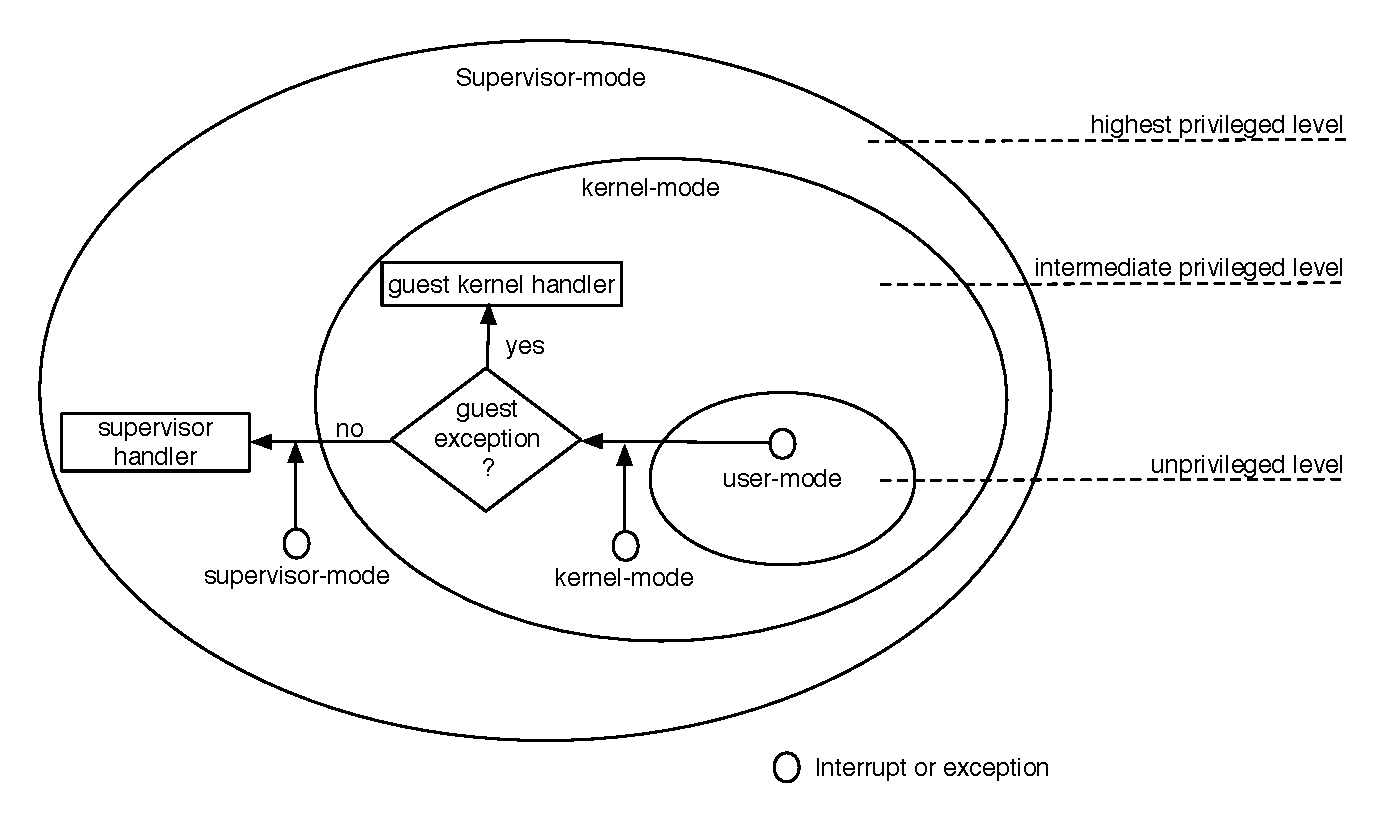
\includegraphics[width=0.6\textwidth]{chapter2/figures/onion}
	\caption{Supervisor privileged level for hypervisor execution.}
	\label{fig:onion}
\end{figure}


\subsubsection{2-Stage TLB Translation}
\label{subsection:tlb}

Processors targeting GPOSs rich in features must support a memory management unit (MMU) to provide a virtual memory mechanism. Thus, the OS can implement memory isolation between processes increasing software reliability and security. Translation look-aside buffer (TLB) is a common hardware construction to assist MMU, which works like a page table cache. High performance processors can automatically performs page walks in the page table when a TLB miss occurs, i.e., the target address is not found in TLB. However, simpler processors will trap the OS in this situation. Thus, the OS must handle a TLB exception to reconfigure the TLB cache. In a virtualized system, the hypervisor must virtualize the MMU keeping the guest OSes isolated from each other, which requires a second stage of address translation. Figure \ref{fig:ipa} shows the difference between virtual memory translation in a non-virtualized versus a virtualized system. In a non-virtualized system, the OS translates virtual addresses (VAs) to physical addresses (PAs) using its page table to configure the TLB. In a virtualized system, VAs are translated to intermediate physical addresses (IPAs), which must be managed by the hypervisor. Processors without the proper virtualization support require the hypervisor to implement a technique called shadow page tables that keeps the correct translation from IPA to PA. Figure \ref{fig:shadow} represents the difference between an OS page table and a hypervisor shadow page tables. When using this technique, the guest OS still manages its page tables, but it cannot configure the processor's TLB directly. The hypervisor handles the page faults reading the address mapping from the guest OS and creating its shadow page table. This second-stage address translation performed by software generates an excessive number of hypervisor exceptions, since, the TLB configuration involves privileged instructions. Again, the number of exceptions can be reduced using hypercalls. 

%\begin{figure}[!hbtp]
%	\centering
%	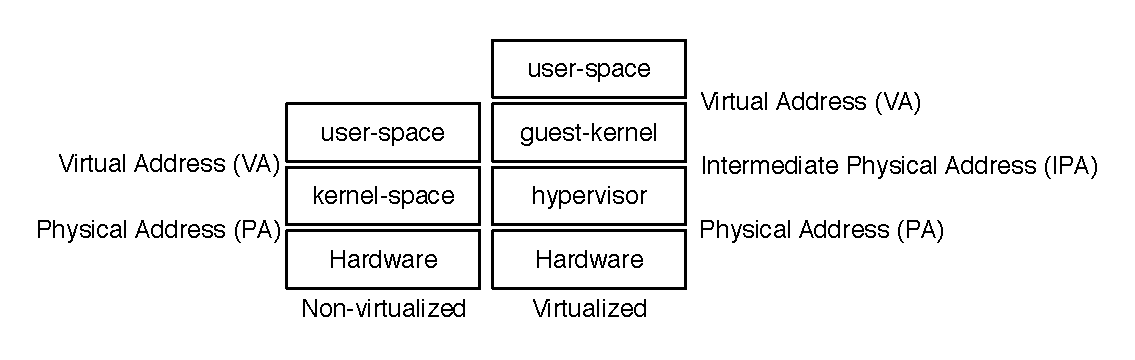
\includegraphics[width=0.9\textwidth]{chapter2/figures/ipa}
%	\caption{Non-virtualized versus virtualized virtual memory address translation.}
%	\label{fig:ipa}
%\end{figure}

\begin{figure}[!hbtp]
\centering
\subfigure[Non-virtualized versus virtualized virtual memory address translation.]{
    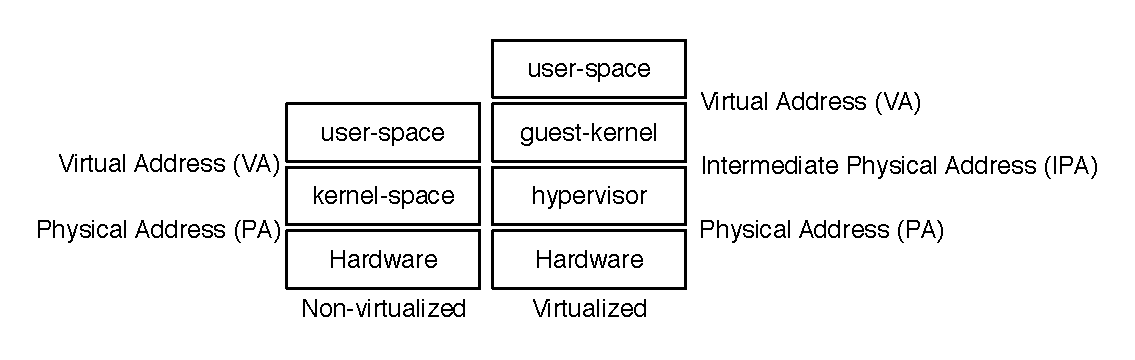
\includegraphics[width=.7\textwidth]{chapter2/figures/ipa}
    \label{fig:ipa}
}

\subfigure[OS page table versus hypervisor shadow page tables.]{
    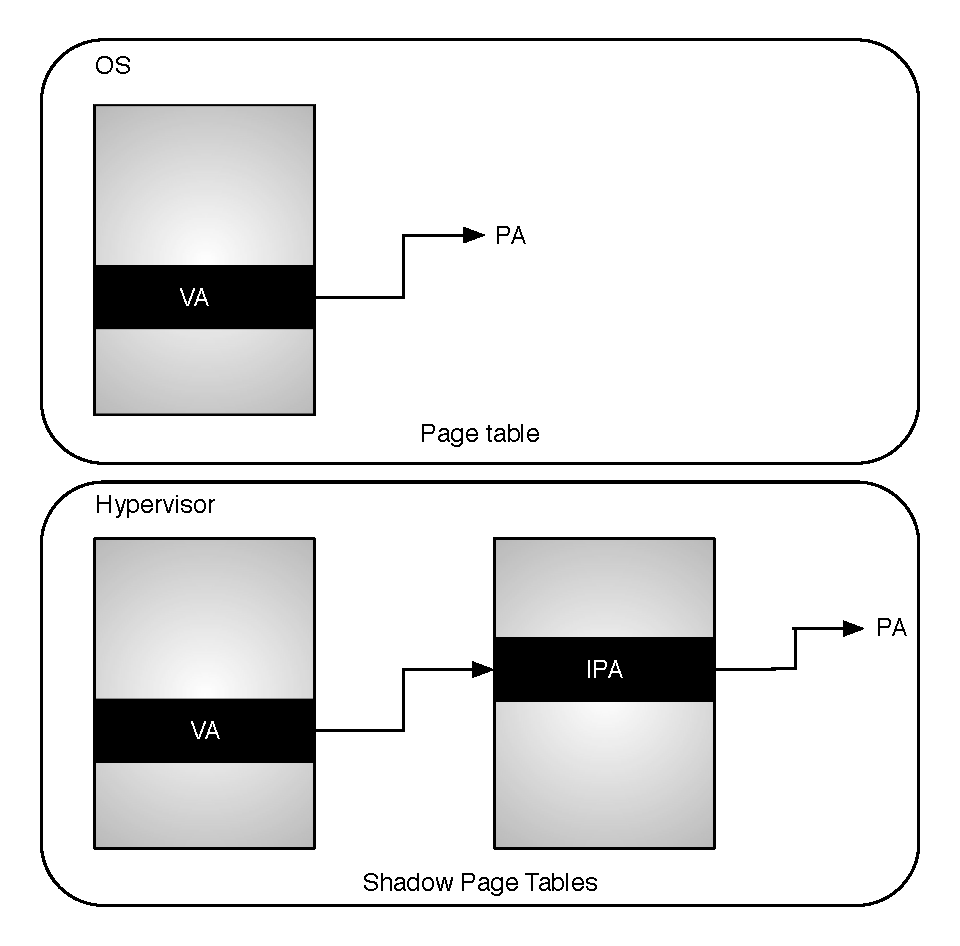
\includegraphics[width=.5\textwidth]{chapter2/figures/shadow-page-table}
    \label{fig:shadow}
}
\captionsetup{justification=centering}
\caption{Memory virtualization approaches in non-virtualized versus virtualized systems.}
%\label{}
\end{figure}


Current virtualization extensions for embedded processor families, like MIPS and ARM, implement a second-stage TLB translation in hardware. Essentially, the hardware performs the translation from IPA to PA without software intervention. The hypervisor still manages its page table mapping IPA to PA. However, the guest OS is allowed to configure directly the TLB. This is possible because the two TLB stages are configured from different processor modes. For example, the hypervisor (supervisor-mode) configures the second-stage TLB while the guest OS (kernel-mode) configures the first-stage TLB. The resulting PA is generated by the hardware combining both TLBs. This mechanism decreases the number of hypervisor exceptions drastically, since the guest OS directly manages  its TLB while decreasing the hypervisor complexity. 

%\begin{figure}[!hbtp]
%	\centering
%	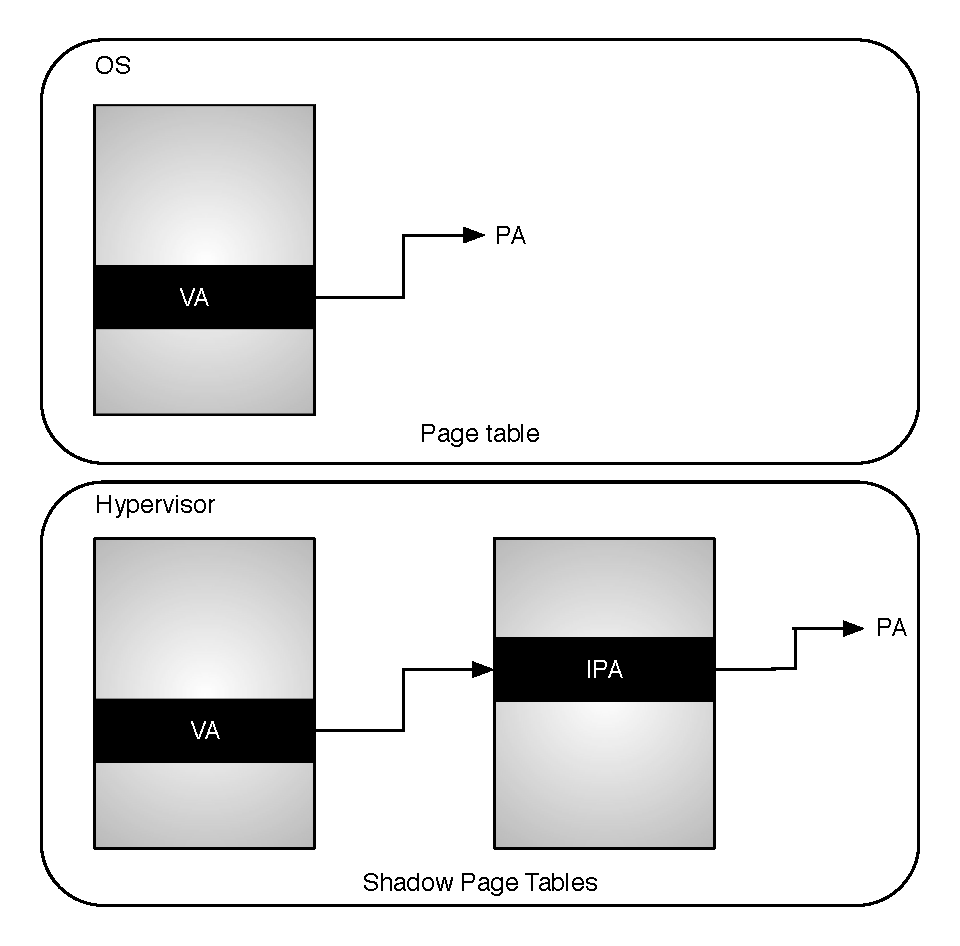
\includegraphics[width=0.4\textwidth]{chapter2/figures/shadow-page-table}
%	\caption{Page table versus shadow page table.}
%	\label{fig:shadow}
%\end{figure}



\subsubsection{Directly Mapped I/O}
\label{subsection:interrupt}

In some cases, it is desirable to map a hardware device directly to a guest OS, e.g., a serial port or a USB device could be directly handled by a guest OS. However, in processors without proper virtualization support, all interrupts are handled in kernel-mode forcing the hypervisor to handle all interrupt sources. This prevents an efficient implementation of a directly mapped I/O. 

One desired feature of a virtualization extension module is the capability of a hypervisor to map an interrupt source to a designed guest OS. For example, an interrupt used as system timer for guest OS scheduling purposes could be directly mapped, avoiding hypervisor intervention during the guest context-switch. Directly mapped devices require the hypervisor to configure an entry in its page table mapping the physical device address to the intermediate physical address (see Subsection \ref{subsection:tlb}) expected by the guest OS. Still, it must map the associated interrupts to the guest OS. Thus, the guest OS will receive  interrupts and read or write to the device without any hypervisor intervention. 


\subsection{I/O Virtualization}
%colocar referência para i/o overhead.
%referencia para IOMMU

There are different ways to manage I/O on a virtualized platform. On a platform without hardware-assisted virtualization, the hypervisor must implement device drivers for all peripherals in use, dealing directly with the system’s I/O. This technique is used in para-virtualized hypervisors. Thus, the device drivers at the operating system level are substituted by para-virtualized device drivers. Beyond to the disadvantage of modifying the OS's I/O subsystem to support para-virtualization, hypervisor intervention in I/O increases the virtualization overhead \cite{Waldspurger2012}. A directly mapped I/O can be used to improve the I/O performance on guest OSs, as explained in the Subsection \ref{subsection:hardware-assisted}. However, it lacks correct support for dynamic memory access (DMA) technique. DMA allows a peripheral to have direct access to the main memory. In a virtualized platform, the hypervisor re-maps the guest OS's memory addresses causing DMA devices to fail. Additionally, this is a security hole since a guest OS can use the DMA to transfer data to another guest OS's memory. Thus, the hypervisor must deny access to the guest OSs from the DMA controller, and to implement a para-virtualized mechanism to allow DMA to such systems. 

Modern processors with proper hardware support for virtualization implement a input–output memory management unit (IOMMU), as supported by the x86 family. IOMMU works similar to the processor's MMU (see Subsection \ref{subsection:tlb}). However, it translates memory accesses performed by devices instead of by the processor. Figure \ref{fig:iommu} compares IOMMU to the MMU. The IOMMU can solve the problem of memory re-mapping on virtualized platforms since the hypervisor can map the DMA addresses to the correct physical address. Additionally, it can avoid the security hole on DMA since it provides memory protection from peripheral read/write in a similar way that MMU provides spatial isolation.

\begin{figure}[!hbtp]
	\centering
	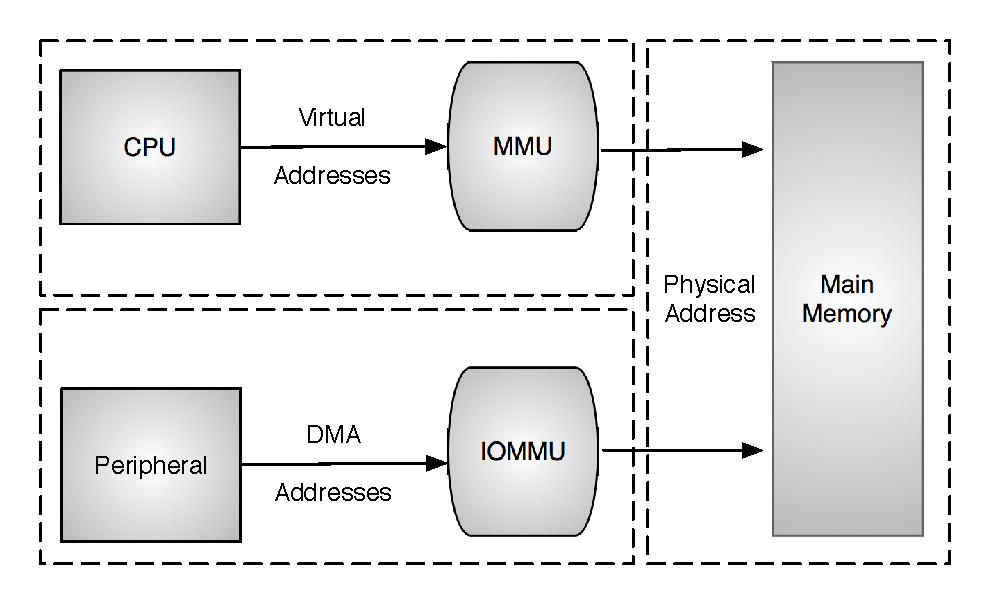
\includegraphics[width=0.55\textwidth]{chapter2/figures/IOMMU}
	\caption{Comparison of the IOMMU to the MMU.}
	\label{fig:iommu}
\end{figure}

Unfortunately, IOMMU is not present on all architectures of the current generation of hardware-assisted virtualization for embedded processors. For more details, Section \ref{section2:future} discusses the evolution of virtualization on embedded systems.


\section{Problems Caused by Virtualization}
\label{section:virt_challenges}

This section gives a brief introduction of two important problems faced in virtualized platforms: the hierarchical scheduling problem (Subsection \ref{subsection:twolayers}) and the lock the holder preemption problem (Subsection \ref{subsection:holder}). Chapter \ref{chapter:vtmodel} explains how the virtualization model proposed by this dissertation avoids this problems.

\subsection{The Hierarchical Scheduling Problem}
\label{subsection:twolayers}

As mentioned in the Subsection \ref{section:es}, real-time is a key feature in many ESs. Enabling real-time support on virtualized platforms causes the hierarchical scheduling problem, also known as two layers scheduling problem. A hypervisor schedules Virtual CPUs (VCPUs), and a guest RTOS executing in a VCPU schedules its processes or tasks. Even ensuring real-time characteristics at the VCPU level, it is difficult to ensure real-time execution to the tasks over the RTOS. However, if VM and hypervisor use proper real-time algorithms, the system can be modeled as a hierarchy of schedulers, and its real-time performance can be evaluated by using hierarchical scheduling analysis techniques \cite{cucinotta2009}.

One reason to use virtualization is to allow for the coexistence of different guest OSs designed for different purposes executing in the same system. For example, a \emph{general-purpose OS} (GPOS) executing along with a legacy RTOS. However, different OSs have different characteristics, e.g., RTOSs privileges real-time over throughput performance. A hypervisor for ESs must be flexible enough to deal with these conflicting characteristics. Thus, more effective approaches should be taken to deal with the two layer scheduling problem. 

Some authors, e.g., Kiszka et al. \cite{kiszka2009}, propose the implementation of hypercalls to allow the guest OS to inform to the hypervisor of its time constraints. Other approach is the use of compositional scheduling as proposed by Lee et al. \cite{Lee2012}. Additionally, an alternative adopted by this dissertation is to perform the scheduling of real-time tasks directly by the hypervisor, i.e., avoiding the two layer scheduling problem and performing a strong temporal separation between general-purpose guest OSs and real-time entities.


\subsection{Lock Holder Preemption Problem}
\label{subsection:holder}

The Lock Holder Preemption (LHP) problem in a virtualized environment happens if a guest OS executing in a SMP configuration is preempted while its kernel is holding a spinlock. Spinlocks are a synchronization primitive widely used in OS's kernels. With spinlocks, a thread waiting to acquire a lock will wait actively monitoring the lock \cite{mitake2012}. As this lock remains, any other VCPU from the same guest trying to acquire this lock will have to wait. Spinlocks imply active waiting, thus, the CPU time is wasted resulting in serious performance and real-time degradation. The LHP problem is possible even if two or more VCPUs execute on a single physical CPU concurrently.

Several approaches were proposed to deal with the LHP problem. The VMWare hypervisor\footnote{http://www.vmware.com/} employs the co-scheduling technique \cite{ousterhout1982}, consisting of a scheduler that tries to execute processes communicating with each other in the same time slice, thus, reducing the chances of blocking. Uhlig et. al. \cite{uhlig2004} proposed a full-virtualized and a para-virtualized technique to deal with the problem. In the full-virtualized technique, the authors consider that the spinlocks are always acquired and released in kernel mode. Thus, the hypervisor never preempts the guest OS when executing in kernel mode, avoiding the LHP problem. Their para-virtualization technique consists of a hypercall to be invoked when entering in spinlock and another hypercall to be invoked when leaving the lock. Thus, the hypervisor knows when a VCPU is in a spinlock and should not preempt it. 

In ES, the main consequence of the LHP problem is the impact in real-time responsiveness. Thus, the LHP should be carefully considered when designing a virtualized ES.


\section{Virtualization for Embedded Systems}
\label{section:ev}

Virtualization is a widespread technology for enterprise and workstation applications, but, it is a relatively new concept in the ES area. The importance of virtualization for ESs is due to its ability to address some of the growing challenges in this area, e.g., the increasing software complexity and time-to-market. One advantage of virtualization is its ability to support heterogeneous operating-system environments to address conflicting requirements such as high level APIs, real-time support or legacy software. The architectural abstraction offered by virtualization allows for migration of multicore guest OSs to virtualized single core systems essentially without modification. Security is another important motivation, since, virtualization can enable a strong spatial separation between the guest OSs \cite{HeiserRole}. 
Virtualization as deployed in the enterprise environment cannot be directly used in ESs. Although ESs are starting to implement some features of general-purpose systems, some differences remain. ESs still present critical real-time constraints and frequently have resource constraints, such as reduced battery capacity, memory and processing power. Thus, virtualization in the ES world is a different challenge than that faced in the enterprise environment. To distinguish server virtualization from embedded system virtualization, the term embedded virtualization is used. Additionally, in this dissertation the term virtualization refers to embedded visualization unless stated otherwise.

This dissertation focuses on embedded systems that require large software stacks to implement their functionalities. These systems can use virtualization to meet these requirements. In addition, the proposed virtualization techniques presented in this dissertation can be used to improve real-time responsiveness and increase security on ESs. Some examples of ES candidates are customer electronics (CE) like smart phones, tablets, set-up box among others. Moreover, enterprise and industrial electronic devices such as network devices (routers and switches) may apply embedded virtualization. Recently, virtualization for IoT devices emerged as a trend. The main advantage of virtualization on IoT is security. Hypervisors can provide memory isolation between applications and implement a Root of Trust software base, which means an environment where the hypervisor guarantees the authenticity of the virtual machines. 

\section{Past, Present and Future of Embedded Virtualization}
\label{section2:future}

Roughly ten years ago, virtualization started to move to the ESs field. At that moment, embedded virtualization was ruled by hypervisors that adopted para-virtualization to overcome the performance issues of full-virtualization. Though some popular hypervisors used for server computing were adapted for embedded systems, other hypervisors were developed from scratch. Some of these hypervisors are still in use, and they will be discussed in Chapter \ref{chapter:stateofart}. These hypervisors were especially designed to deliver virtualization in embedded systems, but in a lightweight way, and implement techniques to improve the real-time responsiveness along with memory separation. 

With the advance of the semiconductors and their decreasing cost, it is possible to implement hardware support for virtualization on embedded processors affordably. The first embedded processors with hardware-assisted virtualization emerged around five years ago. The possibility of implementing full-virtualization without the performance penalties of the past motivated the appearance of newer hypervisors. The current stage of embedded virtualization allows full-virtualization of the CPU combined with para-virtualized I/O. Thus, hybrid hypervisors combine full and para-virtualization. In a few years, proper support for IOMMU on embedded processors will allow for high performance communication between guests using the DMA hardware. 

In the next five years, virtualization will increasingly be used in embedded systems \cite{security-prpl}. Virtualization will not be restricted to powerful embedded devices, but will also be used in IoT devices, primarily motivated by security concerns. Thus, embedded hypervisors will need to execute in devices with extreme hardware restrictions. Small footprint and lightweight execution will still be important.



